\author{Fabrizio}
The STM32D407VG-Discovery board is equipped with a MP45DT02 MEMS microphone and a CS43L22 DAC for audio acquisition and processing. In this project, we will use these devices to detect the sounds' frequency, which will determine the commands given to the robot.

\subsection{The MP45DT02 microphone}
The MP45DT02-M is a compact, low-power, topport, omnidirectional, digital MEMS microphone. It's soldered on the top of the STM32F407G-DISC1 board, in the bottom-right corner.
\begin{figure}[H]
	\centering
	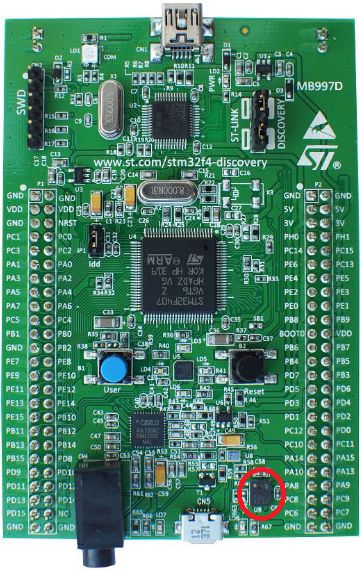
\includegraphics
	{files/images/board_view}
	\caption{View of the upper surface of the board, with the microphone highlighted in the circle.}
\end{figure}

In its bottom surface, it has 6 pins:
\begin{enumerate}
	\item \textbf{GND} - Connected to the GND of the board
	\item \textbf{LR} - Channel selection: used because the microphone is designed to allow stereo audio capture. If it is connected to GND, the MP45DT02 is placed in "left" channel mode: a sample is latched to the data output pin (PDM) on a falling edge of the clock, while on the rising clock edge, the output is set to high impedance. If the LR pin is connected to Vdd then the device operates in "right" channel mode and the MP45DT02 latches it's sample to PDM on a clock rising edge, setting the pin to high impedance on the falling edge of the clock.
	\item \textbf{GND} - Connected to the GND of the board
	\item \textbf{CLK} - Synchronization input clock: this pin is connected to the PB10 port of the board. The clock signal determines the sampling frequency.
	\item \textbf{DOUT} - PDM Data Output. Connected to the PC03 pin of the board's GPIO.
	\item \textbf{VDD} - Power supply.
\end{enumerate}

\begin{figure}[H]
	\centering
	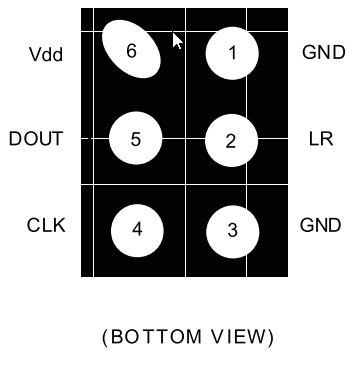
\includegraphics
	{files/images/mic_bottom_pins}
	\caption{Pins on the bottom of the microphone.}
\end{figure}

\subsection{Overview on sound acquisition and processing}
The sound is acquired by the microphone, and the communication with it happens through I2C.\\
The microphone acquires data in PDM format: each sample is a single bit, so the acquisition is a stream of bits; an high amplitude is represented with an high density of '1' bits in the bitstream. \\
The sampling frequency of the ADC is 11000 Hz. \\
In order to process the data, it has to be converted in PCM format: this is done by doing \textbf{CIC filtering}, with a decimation factor of 16 (each 16-bits sequence of 1-bit PDM samples is converted in one 16-bit PCM sample).\\
Then, an FFT analysis is performed on 4096 samples at a time to extract the fundamental frequency and the amplitude of the sound.

\subsection{Microphone initialization}
The initialization of the sound acquisition system comprehends several steps:
\begin{enumerate}
	\item SPI, DMA and General Purpose ports B and C are enabled through RCC
	\item GPIO ports are configured in \textit{Alternate} mode
	\item SPI is set to work in I2S mode
	\item interrupt handling for DMA is configured
	
\end{enumerate}

\subsection{Sound acquisition and processing}
Each time a new sample is read, the functions in the Microphone object:
\begin{enumerate}
	\item Read 16 bits from SPI and transfer them in RAM through DMA
	\item  Convert 16 PDM samples in one 16-bit PCM sample via \textbf{CIC filtering} with a decimation factor of 16
	\item Perform FFT through the \textit{arm\_cfft\_radix4\_f32}  module
	\item Calculate amplitude of each frequency with the \textit{arm\_cmplx\_mag\_f32} module
	\item Calculate the Harmonic Product Spectrum to find the fundamental frequency (and its amplitude) in the vector
	\item Store the values of the fundamental frequency and its amplitude in dedicated variables, then call the \textbf{callback function} to react to the detected frequency.
\end{enumerate}
In our project, the \textbf{callback function} is in charge of producing commands to the engines when the frequency of the last acquired sample is in some specified ranges.

\subsection{The Microphone.cpp driver}
Sound acquisition and samples' processing is performed by the \textbf{Microphone.cpp} driver. \\
This driver was originally developed by Riccardo Binetti, Guido Gerosa and Alessandro Mariani, but it has been improved by Lorenzo Binosi and Matheus Fim in their \textit{Digital Guitar Tuner} project. \\
For our project, we have also made some changes to the driver, such as including the frequency recognition feature in the driver itself and adding the amplitude recognition of the audio samples. \\
The usage of the driver is very simple:
\begin{enumerate}
	\item Add the \textbf{Microphone.cpp} and \textbf{Microphone.h} files in the folder of the other source files of the project, and add the \textit{Microphone.cpp} entry in the \textbf{SRC} line of the makefile
	\item Add the \textit{\#include "Microphone.h"} line at the start of the source file that will use the Microphone object
	\item Declare 2 float32\_t variables to store the frequency and the amplitude of the last acquired sample
	\item Define a void callback function without parameters
	\item Create a Microphone object using the \textit{Microphone::instance()} method
	\item Initialize the microphone with the \textit{mic.init(\&callback, \&freq, \&amplitude)} method, passing to it the addresses of the 2 variables and of the callback function
	\item Use the \textit{start()} method of the Microphone object to start acquiring and processing samples. This method is non-blocking (operations are performed in other threads).
\end{enumerate}
Each time a new 16-bit PDM sample has been acquired, the driver will perform an FFT analysis on it and will write the frequency and the amplitude of the sample in the chosen variables, then the callback function will be called automatically. This process will be iterated continuously until the \textit{stop()} function of the Microphone object is called.